\documentclass[a4paper,11pt]{article}

% Packages
\usepackage[utf8]{inputenc}
\usepackage[english]{babel}
\usepackage{amsmath, amssymb}
\usepackage{graphicx}
\usepackage{booktabs}
\usepackage{float}
\usepackage{caption}
\usepackage{siunitx}
\usepackage[hidelinks]{hyperref}
\usepackage{fancyhdr}
\usepackage[frozencache,cachedir=_minted-cache]{minted}
\usepackage{enumitem}
\usepackage{titlesec}
\usepackage{multicol}
\usepackage{geometry}
\geometry{margin=2cm}

% Header/Footer
\pagestyle{fancy}
\fancyhf{}
\fancyfoot[L]{Marc Toiflhart, Sebastian Maier}
\fancyfoot[C]{\thepage}
\fancyfoot[R]{Högskolan i Halmstad}
\fancyhead[L]{\nouppercase{\leftmark}}

% Document
\begin{document}

% Title Page
\begin{titlepage}
    \centering
    
\includegraphics[width=5cm]{Resources/hogskolan-halmstad-logo.png}\\[0.5cm]
    Högskolan i Halmstad \\[0.2cm]
    Biometric Recognition Laboratory – Fingerprint \\[1.5cm]
    
    \hrule
    \vspace{0.4cm}
    {\LARGE \textbf{Report}}\\[0.2cm]
    \textbf{Fingerprint Recognition}\\[0.2cm]
    \hrule
    \vspace{1.2cm}

    \textbf{Authors:} Marc Toiflhart, Sebastian Maier\\[0.3cm]
    \textbf{Supervisor:} Kevin Hernández Diaz\\[0.3cm]
    \textbf{Date:} \today
    \vfill
\end{titlepage}
\newpage

% Summary
\section*{Summary}
In this lab we worked with fingerprint images and studied how biometrics systems detect special points in fingerprints. We learned about ridge and valley structure, image quality, and enhancement techniques. We also tested a detection algorithm in MATLAB and checked how filtering and interpolation improve the fingerprint image. At the end, we calculated pixel values by hand to better understand the enhancement process.

% Exercise 1
\section{Exercise 1}
\textbf{Introduction:}  
In this exercise we run the fingerprint detection algorithm and analyse the ridge width and the quality of different fingerprint areas. We also identify parts where the quality is low.

\subsection{How much width (in mm) has a ridge/valley in a human fingerprint?}
Fingerprints are quasi-periodic with a ridge period (ridge-to-ridge distance) of about
\SI{0.4}{\milli\meter} on average (typically \SI{0.35}-\SI{0.5}{\milli\meter} across fingers).
Assuming roughly symmetric ridges and valleys, a single ridge (dark line) is
about \SI{0.2}{\milli\meter} wide and a valley (bright gap) about \SI{0.2}{\milli\meter}.
In the grayscale image, the size of said ridges was meassured in pixels:
$\approx 8$ pixels per ridge period which corresponds to \SI{0.4}{\milli\meter} at \SI{500}{dpi} (\SI{19.685}{px/mm}).

\subsection{How would you describe an area of poor quality of a fingerprint?}

We define poor quality as regions where one or more hold:
\begin{enumerate}[itemsep=2pt,topsep=2pt]
    \item Low ridge--valley contrast (gray, washed-out appearance).
    \item Orientation instability (rapidly varying or incoherent ridge flow).
    \item Structural corruption (smudges, scars, cuts, dryness/wetness artifacts).
    \item High noise and broken/merged ridges leading to spurious minutiae.
\end{enumerate}
Operationally, these appear where the direction field is noisy and symmetry filter responses are weak or scattered.

\subsection{Indicate the parts of the fingerprint that has poor quality}

The above described errors can be found in the \textbf{lower third} part and at the \textbf{top right corner} of \autoref{fig:gradient_levels}.
\noindent
This is underlined by the \textbf{gradient vectors} in the said parts of the image: the magnitude is significantly lower, thus indicating that the qualtiy of the structure in these parts is compromised.

\begin{figure}[H]
    \centering
    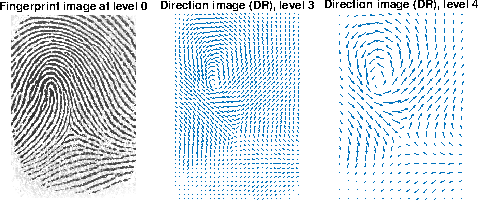
\includegraphics[width=0.75\textwidth]{figures/latex_figs/fig01_image_DR_L3_L4.pdf}
    \caption{Gradient Image of the unenhanced fingerprint}
    \label{fig:gradient_levels}
\end{figure}

% Exercise 2
\section{Exercise 2}
\textbf{Introduction:}  
Here we activate fingerprint image enhancement and compare the detected points before and after the enhancement. We also study how the enhancement algorithm works.

\subsection{Was enhancement of the fingerprint successful?}
Yes. We judge success by (i) higher ridge--valley contrast, (ii) smoother direction field, 
(iii) stronger, localized core/delta responses, and (iv) fewer spurious minutiae.
These criteria are met when comparing pre/post figures:

\begin{figure}[H]\centering
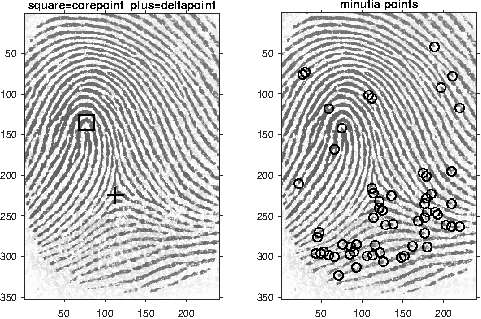
\includegraphics[width=.42\textwidth]{figures/latex_figs/fig50_S_and_M_no_enhance.pdf}\hfill
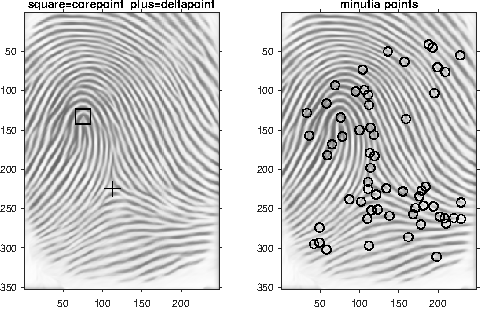
\includegraphics[width=.42\textwidth]{figures/latex_figs_enhanced/fig51_S_and_M_enhanced.pdf}
\caption{Extraction overlays without (left) and with (right) enhancement. Post-enhancement shows cleaner ridge flow, tighter core/delta localization, and a more stable minutiae set.}
\end{figure}

To underline the difference in quality between the original and the enhanced fingerprint, the number of falsely classified minutiae was counted:
\begin{itemize}
    \item Original: 46
    \item Enhanced: 22
\end{itemize}

It is hereby evident, that the enhancement was indeed successful.

\subsection{Find out and explain how the enhancement algorithm works}

The enhancement algorithm improves the fingerprint image so that the ridges become clearer and easier to follow.  
It is based on \textbf{directional Gaussian filtering}, also called \textbf{orientation-steered enhancement}.

\begin{enumerate}[itemsep=2pt,topsep=2pt]
    \item \textbf{Orientation estimation:}  
    For each small region of the image, the algorithm estimates the local ridge direction~$\theta(x,y)$ by analysing image gradients. This gives the dominant orientation of the ridge flow.

    \item \textbf{Directional filtering:}  
    Several \textbf{directional Gaussian filters} are applied to the image, each oriented at a different fixed angle (for example 30°, 60°, 90°, 120°, 150°).  
    Each filter smooths the image mainly \emph{along} its direction (using a large $\sigma_\parallel$) and less \emph{across} it (small $\sigma_\perp$).  
    This reduces noise and connects broken ridge segments.

    \item \textbf{Combination of filtered images:}  
    After all directions are filtered, the algorithm selects, for every pixel, the output of the filter that best matches its local ridge direction~$\theta(x,y)$.  
    In this way, every pixel is enhanced using the filter that follows its true ridge orientation.  
    The result is a combined image where ridges are continuous, valleys are clean, and background noise is suppressed.

    \item \textbf{Effect:}  
    The final enhanced image has stronger contrast and smoother ridge flow, which improves the accuracy of the later steps that detect core, delta, and minutiae points.
\end{enumerate}


\begin{figure}[H]\centering
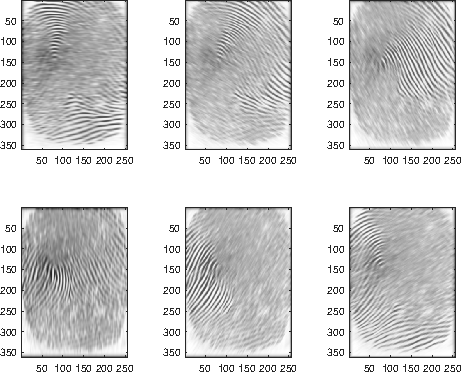
\includegraphics[width=.6\textwidth]{figures/latex_figs_enhanced/fig55_filtered_images.pdf}
\caption{Intermediate enhancement results: progressive, orientation-aligned smoothing increases ridge continuity and contrast.}
\end{figure}

% Exercise 3
\section{Exercise 3}
\textbf{Introduction:}  
In this exercise we focus on the linear interpolation step. We choose pixels and compare the enhanced value with the filtered images to understand the weights and interpolation.

\subsection{Computation}

Two example pixels were analysed to illustrate how the linear interpolation between directional filters is performed.

\paragraph{Point 1: $(r,c) = (152,173)$}
\[
\texttt{out} =
\begin{bmatrix}
67.05 & 186.83 & 181.98 & 135.74 & 147.33 & 173.10 & 180.79
\end{bmatrix}^\mathsf{T}
\]
The local orientation is $\phi = 67.05^\circ$, which lies between the filters at $60^\circ$ and $90^\circ$.
\[
w_{60} = \frac{90 - 67.05}{30} = 0.765, \quad
w_{90} = \frac{67.05 - 60}{30} = 0.235,
\]
\[
I_\text{enh}(152,173)
= 0.765\times135.74 + 0.235\times147.33
\approx \mathbf{138.5}.
\]

\paragraph{Point 2: $(r,c) = (198,39)$}
\[
\texttt{out} =
\begin{bmatrix}
123.10 & 169.02 & 170.32 & 168.07 & 155.50 & 107.66 & 145.14
\end{bmatrix}^\mathsf{T}
\]
Here, $\phi = 123.10^\circ$ lies between $120^\circ$ and $150^\circ$.
\[
w_{120} = \frac{150 - 123.10}{30} = 0.897, \quad
w_{150} = \frac{123.10 - 120}{30} = 0.103,
\]
\[
I_\text{enh}(198,39)
= 0.897\times107.66 + 0.103\times145.14
\approx \mathbf{111.6}.
\]

The calculated intensities are an \textbf{exact match} to the intersities optained in the combined grayscale image.

\paragraph{Interpretation}
In both cases, the enhanced gray level is obtained as a weighted average between the two filtered images whose orientations are closest to the local ridge direction.  
This ensures that each pixel is enhanced along its real ridge flow, even when the ridge angle lies between the discrete filter directions.

\end{document}